\section{Preprocessing}
The bag of words model used by our classifiers is a good way to represent the data found in the given training documents. However this feature representation is prone to very high dimensions if not handled well due to the large number of possible combinations in words. 

According to a recent survey performed by Google and Harvard, there are approximately 1,022,000 different words in the English language \cite{google2010words}. While we do not expect to find all possible words in the document corpus, a large number of them will be found along with their derivations in the form of spelling mistakes and grammatical variations (e.g.{\it they're} and {\it theyre}). Other non-English words such as html code, URLs and nonsensical data such as GPG keys will also be found within the documents.

Most of these words will provide no benefit to the classifier and in most cases will even harm the classifier's performance. It is therefore of utmost importance that noise in the text is filtered out and the number of word combinations is reduced to the most representative, yet minimal subset of the available words. The following steps are taken to do this:
\begin{itemize}
	\item Smart Email Parsing
	\item Simple Text Processing Techniques
	\item Domain Extraction
	\item Stemming
	\item Feature Selection based on Document Frequency
\end{itemize}

Each of these steps contribute towards achieving a higher accuracy and performance in the classifier and will be described in detail in the sections below.

\subsection{Email Parsing}
As a first preprocessing step, we modify the parsing of the email structure.
The provided emails sometimes contain metadata which is very redundant w.r.t. to the number of contained words, e.g. all will have a "From" line but also if an email has metadata is independent from its class label, i.e. the classifier should not that all mails that have metadata are spam.
Furthermore mails do not always consist of just text but also have attachments or their textual content is supplied as plain text or beautified with HTML markup.

In a first step, we strip the metadata from the email so that only give the content of the mail to the classifier.
This reduces the size of data passed on to the classifier as most terms in the metadata are either common among all emails, e.g. the names of the header lines (``From'', ``Content-Type'', \dots), or are unique to the mail like the date of sending or the message-id.
From the metadata we extract some basic information like the encoding or if it is a multi-part email for further processing.

If the mail is split in multiple parts, we want to extract only the parts which contain text as we cannot infer information of the \emph{base64} representation of images or other binary attachments.
These binary attachments would only add a large number of words of a length of 76 characters \cite{rfc2045} to the index which are very uncommon in other mails as images are compressed data with a high entropy.
Another problem that is solved by adding handling multiple is the recursive parsing of attached emails that have textual content and may have multiple parts again inside so that we are now stripping down the inner mails to their actual content too.

Furthermore not all text is encoded in the same encoding as the email itself, e.g. the main text could be encoded as Base64 which would not reveal the actual words when just splitting the mail into words by separating at each space.
Another typical encoding is quoted-printable which only transforms non-ASCII characters into another format but leaves all ASCII characters intact.
Handling these encoding turns meaningless, long character sequences into words that are present in other mails.

As a final parsing step in the email handling we are stripping all HTML from the mails to remove all HTML tags from our word index.
This markup is not displayed to the user and does not carry any content that will be some sort of advertising.

\todo{Improvement?}

\subsection{Simple Text Processing Techniques}

A number of simple processing techniques are used to conflate incoming strings that represent the word together. Although the email parser is built in such a way as to strip out html content where possible, a number of artefacts could still linger in the data which could cause noise and incorrectly distinguish variations of the same word. Because it is not the parsers job to perform this form of filtering, a separate step is taken to perform simple text processing tasks before passing them on the later pre-processing stages.

All incoming words that are composed purely of symbols (i.e. no numbers or letters) are simply discarded as they are most commonly noise in the data that does not represent anything in the corpus. Without this step, the number of features used by the classifier would grow substantially as a large number of "rubbish" symbols are included as part of the feature set. Additionally, all remaining words will have ally symbols stripped, this prevents variations in words like {\it they're} and {\it theyre} from treated as different features.

As a second step, all valid incoming words are simply reduced to lower-case format. The same word in different cases should not be distinguished from one another during classification so it is important that e.g. {\it Bristol} is considered the same as {\it bristol}.

Finally, variations in number representations (e.g. 4,000 and 4000) are detected using regular expressions and conflated to a single representative feature "9999". We do this because allowing all possible number combinations each a unique feature will increase the dimensionality substantially and rarely contribute to classification performance - it can most often be considered noise. Doing this also provides some assurance that we do not overfit our classifier to the training set with specific numeric combinations.

\subsection{Domain Extraction}



\subsection{Stemming}
Most words in the English language are derived from a {\it morphological root} word that contains no prefixes or suffixes and conveys a very similar meaning to its derivation. A simple example of this is {\it subscriber} and {\it subscription} with their morphological root {\it subscribe}. 

If we can reduce all incoming words into their root form, we would be able to substantially reduce the number of dimensions for our model while also ensuring that words representing the same underlying feature are stored under the same value.

Unfortunately, such a task is quite hard and would probably require the creation of a very large lookup table for each word in the English language along with its root. This is due to the fact that the English language is not a formal language and hence does not follow a strict set of rules. 

We could however, take an approximation of the described process and instead derive the {\it stem} of each word. Like the morphological root, the stem is a representation of a words underlying meaning. However the stem does not guarantee to be a correct English word or generate the right root as its aim is simply to map variations of the same word to the same to item. 

For our Spam Filter implementation, we made use of the Porter Stemmer algorithm \cite{porter1980}, which in the authors words is ``a process for removing the commoner morphological and inflexional endings from words in English process''. In simpler terms, it is capable of removing known suffixes from words passed to it. The Porter Stemmer algorithm is available as open source code under the BSD License and is available in multiple languages, including Java which is made use of in our implementation.

Using the same examples shown before, passing {\it subscriber} and {\it subscribe} to the Porter Stemmer would reduce the words {\it subscribe} and {\it subscriber} to the stem {\it subscrib}. On the other hand, the word {\it subscription} will be wrongly mapped to a different stem - {\it subscript}. The latter is an example of where the approximation fails to produce the correct result, however in general most words passed to the algorithm have shown to produce favourable results.

In terms of the Spam Filter implementation, using Porter Stemming on the given set of training emails reduced the number of words from 24813 words to 18932 stems (both after text pre-processing). This is a substantial reduction in the number of dimensions and plays a crucial role in ensuring that the classifier is able to train with the given documents in a short amount of time and without requiring large amounts of memory. Apart from improving speed and reducing memory, it has also proved to improve classification performance. \todo{include some results - simple example I have is 0.973 with and 0.97 without}.

\todo{Improvement?}

\subsection{Feature selection}
\todo{Is this really preprocessing?}

As the number of features generated by the input data is even very high after the previous preprocessing steps, we are going to minimise its number by trimming features which are (significantly) relevant for the classification quality.

\todo{\dots}

\begin{figure}[h!]
    \centering
    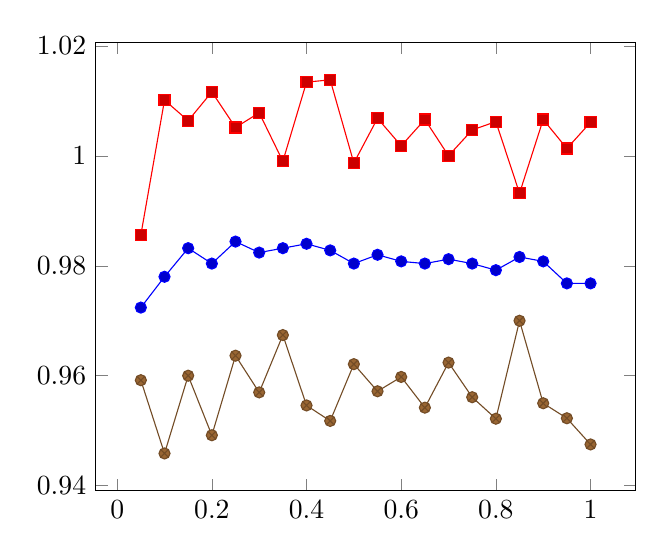
\begin{tikzpicture}
        \begin{axis}
             \addplot+[sharp plot] coordinates {
                (0.05, 0.972400)
                (0.10, 0.978000)
                (0.15, 0.983200)
                (0.20, 0.980400)
                (0.25, 0.984400)
                (0.30, 0.982400)
                (0.35, 0.983200)
                (0.40, 0.984000)
                (0.45, 0.982800)
                (0.50, 0.980400)
                (0.55, 0.982000)
                (0.60, 0.980800)
                (0.65, 0.980400)
                (0.70, 0.981200)
                (0.75, 0.980400)
                (0.80, 0.979200)
                (0.85, 0.981600)
                (0.90, 0.980800)
                (0.95, 0.976800)
                (1.00, 0.976800)
                };
             \addplot+[sharp plot] coordinates {
                (0.05, 0.972400+0.013206)
                (0.10, 0.978000+0.032125)
                (0.15, 0.983200+0.023186)
                (0.20, 0.980400+0.031215)
                (0.25, 0.984400+0.020746)
                (0.30, 0.982400+0.025424)
                (0.35, 0.983200+0.015799)
                (0.40, 0.984000+0.029394)
                (0.45, 0.982800+0.031010)
                (0.50, 0.980400+0.018287)
                (0.55, 0.982000+0.024819)
                (0.60, 0.980800+0.021014)
                (0.65, 0.980400+0.026199)
                (0.70, 0.981200+0.018804)
                (0.75, 0.980400+0.024298)
                (0.80, 0.979200+0.027011)
                (0.85, 0.981600+0.011593)
                (0.90, 0.980800+0.025799)
                (0.95, 0.976800+0.024528)
                (1.00, 0.976800+0.029285)
                };
             \addplot+[sharp plot] coordinates {
                (0.05, 0.972400-0.013206)
                (0.10, 0.978000-0.032125)
                (0.15, 0.983200-0.023186)
                (0.20, 0.980400-0.031215)
                (0.25, 0.984400-0.020746)
                (0.30, 0.982400-0.025424)
                (0.35, 0.983200-0.015799)
                (0.40, 0.984000-0.029394)
                (0.45, 0.982800-0.031010)
                (0.50, 0.980400-0.018287)
                (0.55, 0.982000-0.024819)
                (0.60, 0.980800-0.021014)
                (0.65, 0.980400-0.026199)
                (0.70, 0.981200-0.018804)
                (0.75, 0.980400-0.024298)
                (0.80, 0.979200-0.027011)
                (0.85, 0.981600-0.011593)
                (0.90, 0.980800-0.025799)
                (0.95, 0.976800-0.024528)
                (1.00, 0.976800-0.029285)
                };
    \end{axis}
    \end{tikzpicture}
    \caption{Accuracy w.r.t. upper threshold (lower threshold = 0)}
    \label{p:upperbound}
\end{figure}


\todo{explain what each line in the figure represents and make sure standard deviation is calculated correctly (it should not go above 1.0)..}
